\documentclass[12pt]{article}

\usepackage{jaridocumentation}
\usepackage[table]{xcolor}
\usepackage{tabularx}
\usepackage[utf8]{inputenc}
\usepackage{graphicx}
\usepackage{float}

\begin{document}
 
\title{Gesellschaftsrecht, Erbrecht und Marketing}
\author{Jannick Riond\\
KME V6d SWR}

\maketitle
\newpage
\tableofcontents
\newpage

\section{Gesellschaftsrecht, Kap. 7}
\subsection{Rechtsformen}
\subsubsection{Übersicht der Rechtsformen}
Die in der Schweiz gebräuchlichen Rechtsformen sind:
\begin{itemize}
    \item Einzelunternehmen (Art. 945 f. OR)
    \item Kollektivgesellschaft \textit{KlG} (Art. 552-593 OR)
    \item Kommanditgesellschaft \textit{KmG} (Art. 594-619 OR)
    \item Aktiengesellschaft \textit{AG} (Art. 620-763 OR)
    \item Gesellschaft mit beschränkter Haftung \textit{GmbH} (Art. 772-827 OR)
    \item Genossenschaft \textit{Gen} (Art. 828-926 OR)
    \item Verein (Art. 60-79 OR)
    \item Stiftung (Art. 80-89a ZGB)
\end{itemize}

\subsubsection{Gesellschaftsbegriff}\label{Gesellschaftsbegriff}
Das OR definiert eine Gesellschaft wie folgt:
\begin{Definitionsbox}
"\textbf{Gesellschaft} ist die vertragsmässige Verbindung von zwei oder mehreren Personen zur Erreichung eines gemeinsamen Zwecks mit gemeinsamen Kräften oder Mitteln." (Art. 530 Abs. 1 OR)
\end{Definitionsbox}
Die drei (Tatbestands-)Merkmale einer Gesellschaft sind:
\begin{enumerate}
    \item Die Gesellschaft ist eine \textbf{Personenvereinigung}.
    \item Sie beruht auf einer \textbf{vertraglichen Grundlage}.
    \item Sie dient der \textbf{gemeinsamen Zweckverfolgung}.
\end{enumerate}
\textrightarrow Abgrenzung zur Stiftung die keine Mitglieder hat (Art. 80 ff. ZGB)

\newpage
\subsubsection{Arten von Gesellschaften}
\begin{itemize}
    \item Körperschaften (AG, GmbH, Gen, Verein)\\
    $\hookrightarrow$ Juristische Personen\footnote{Eine juristische Person ist eine vom Gesetz künstlich geschaffene Rechtspersönlichkeit, die unabhängig von natürlichen Personen Träger von Rechten und Pflichten ist.} die selbst rechts- und handlungsfähig sind. Sie schliessen selber Verträge ab und haften mir ihrem Vermögen. Sie haben im rechtlichen Sinne eine \textbf{eigene Persönlichkeit}.
    \begin{figure}[h]
        \begin{center}
            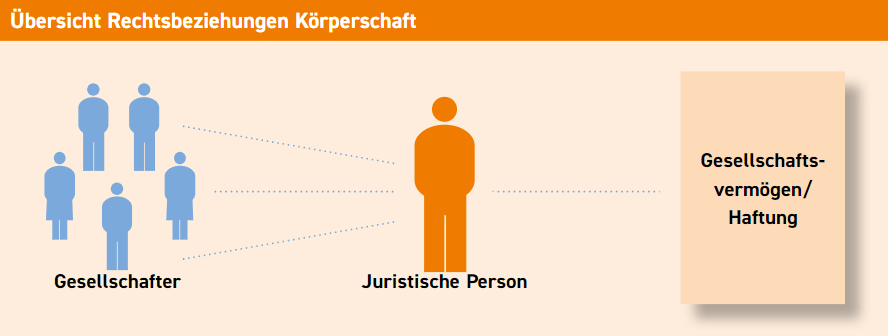
\includegraphics[scale=0.4]{Korperschaften.png}
        \end{center}
    \end{figure}
    \item Personengesellschaften (einfache Gesellschaft, KlG, KmG)\\
    $\hookrightarrow$ Keine Juristische Personen. Träger von Rechten und Pflichten sind die Gesellschafter zusammen. \textrightarrow Rechtsgemeinschaft. Die Gesellschafter haften grundsätzlich \textbf{solidarisch}. (Art. 143 ff. OR)
    \begin{figure}[h]
        \begin{center}
            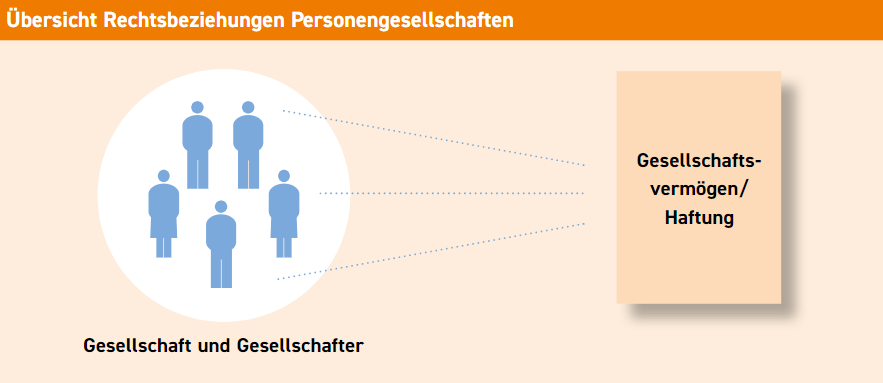
\includegraphics[scale=0.4]{Personengesellschaften.png}
        \end{center}
    \end{figure}
    \item Personenbezogene Gesellschaften und Kapitalgesellschaften\\
    $\hookrightarrow$ Stehen je nachdem entweder das Mitwirken der Personen (wie bei Personengesellschaften, Gen, Verein) oder das mitwirkende Kapital (wie bei AG, GmbH) im Vordergrund.
    \item Handelsgesellschaften (KlG, KmG, AG, GmbH)\\
    $\hookrightarrow$ Sie sind auf Handelsverkehr ausgerichtet.
\end{itemize}

\subsubsection{Wahl der Rechtsform}
Wahlkriterien bei der Entscheidung für eine Rechtsform sind: Unabhängigkeit, Namen, Kapitalbedarf, Gründungskosten, Gewinn- und Verlustverteilung, Geschäftsführung, Risiko, Steuern, Sozialversicherung.

\subsection{Handelsregister und Firma}
\subsubsection{Handelsregister}
\begin{Definitionsbox}
    Das \textbf{Handelsregister} ist eine amtlich geführte und öffentlich einsehbare Datenbank mit Informationen über Gesellschaft und Unternehmen. (Art. 927 ff. OR)
\end{Definitionsbox}

\subsubsection{Inhalte des Handelsregister}
\begin{itemize}
    \item Firma (Name)
    \item Identifikationsnummer
    \item Sitz
    \item Rechtsform
    \item Unternehmenszweck
    \item zur Vertretung berechtigte Personen
    \item eine allfällige Revisionsstelle
    \item Je nach Form: Inhaber, Gesellschafter (und Anteile), Aktienkapital, Nennwert, Mitglieder des Verwaltung, Stammkapital, Mitglieder des Vorstands
\end{itemize}

\subsubsection{Eintragungspflicht}
Zur Eintragung ins Handelsregister ist verpflichtet, \underline{wer als natürliche Person ein Gewerbe betreibt}, das einen
\begin{equation*}
    \text{Jahresumsatz}  \geq 100000
\end{equation*}
hat. (Art. 931 Abs. 1 OR)

\subsubsection{Rechtsfolgen der Eintragung}
Ein Einzelunternehmen welches nicht eingetragen werden muss, darf freiwillig eingetragen werden.
(Art. 931 Abs. 3 OR)

Davon ausgenommen sind allerdings freie Berufe wie Ärzte, Zahnärzte, Ingenieure, Architekten, Rechsanwälte und die Landwirtschaftsbetriebe.

\newpage
\subsubsection{Wirkungen der Eintragungen}
\begin{itemize}
    \item Konstitutive Wirkung (Art. 52 ZGB, Art. 643, 779, 838 OR)\\
    $\hookrightarrow$ (aus lateinisch \textit{constitutus}: "grundlegend", "tragend", "begründend") Manche Gesellschaften (AG, GmbH) entstehen erst mit der Eintragung ins Handelsregister.
    \item Deklaratorische Wirkung\\
    $\hookrightarrow$ Angabe des Rechtsverhältnisses
    \item Publizitätswirkung (Art. 936b OR)\\
    $\hookrightarrow$ Die im Handelsregister eingetragenen Tatsachen gelten als bekannt und wirken gegenüber jedermann.
    \item Schutz der Firma (Name)\\
    $\hookrightarrow$ Mit der Eintragung wird die Firma (Name) der eingetragenen Gesellschaft geschützt.
    \item Betreibung auf Konkurs\\
    $\hookrightarrow$ Im Handelsregister eingetragene Personen und Gesellschaften unterliegen der Betreibung auf Konkurs.
\end{itemize}

\subsubsection{Firmenrecht}
\begin{Definitionsbox}
    In der Rechtssprache bezeichnet der Begriff \textbf{Firma} den Namen eines Unternehmens.
\end{Definitionsbox}
Bei der Wahl der Firma müssen drei Grundsätze beachtet werden:
\begin{itemize}
    \item Firmenwahrheit (Art. 929 Abs. 1 OR \& Art. 944 Abs. 1 OR)\\
    $\hookrightarrow$ Firma muss der Wahrheit entsprechen und dark keine Täuschung verursachen.
    \item Bildung der Firma (Art. 945, 950 OR)\\
    $\hookrightarrow$ Je nach Rechtsform gibt es unterschiedliche Vorschriften zur Bildung der Firma.
    \item Firmenausschliesslichkeit (Art. 946, 951 OR)\\
    $\hookrightarrow$ Firmen müssen sich klar voneinander Unterscheiden. Einzelunternehmen dürfen keine Firma wählen, die in ihrem Ort schon vorhanden ist. Bei Handelsgesellschaften und Genossenschaft gilt die Firmenausschliesslichkeit für die ganze Schweiz.
\end{itemize}

\newpage
\subsection{Einzelunternehmen}
Das Einzelunternehmen ist die Rechtfsorm, bei der ein alleiniger Inhaber ein Geschäft betreibt. Ein Einzelunternehmen ist eine natürliche Person.

Es eignet sich für Kleinunternehmen und personenbezogene Tätigkeiten. Der Inhaber eines Einzelunternehmen kann einfach und schnell Entschlüsse fassen. Der Gewinn gehört ihm allein, dafür trägt er auch die ganze Verantwortung.

\begin{figure}[h]
    \begin{center}
            \includegraphics[scale=0.4]{Übersicht Einzelunternehmen.png}
    \end{center}
\end{figure}

\subsection{Gesellschaften}
\subsubsection{Einfache Gesellschaft (Art. 530 - 551 OR)}
Die einfache Gesellschaft ist die Grundform des schweizerischen Gesllschaftsrechts. Ihre Entstehungsvorraussetzungen, respektive Merkmale haben wir im Kapitel \ref{Gesellschaftsbegriff} thematisiert. 

Sie dient insbesondere als Auffangform für alle Gesellschaften, die nicht die besonderen Voraussetzungen einer anderen Geselschaftsform erfüllen.\\
$\hookrightarrow$ \textbf{Subsidiäre Gesellschaftsform} (Art. 530 Abs. 2 OR)
\begin{figure}[h]
    \begin{center}
            \includegraphics[scale=0.4]{Übersicht Einfache Gesellschaft.png}
    \end{center}
\end{figure}

\subsubsection{Kollektivgesellschaft (Art. 552 - 593 OR)}
Die Kollektivgesellschaft ist die Rechtsform, bei der mehrere natürliche Personen gemeinsam ein kaufmännisches Gewerbe führen.

Sie eignet sich für kleinere Unternehmen, deren Tätigkeit auf mehrere Gesellschafter\footnote{Wobei bei der KlG nur natürliche Personen Gesellschafter werden können.} bezogen sind und keine besonderen Risiken mit sich bringen.
\begin{figure}[h]
    \begin{center}
            \includegraphics[scale=0.4]{Übersicht Kollektivgesellschaft.png}
    \end{center}
\end{figure}

\subsubsection{Kommanditgesellschaft (Art. 594 - 619 OR)}
Die Kommanditgesellschaft ist eine Sonderform der KlG. Sie kennt nämlich zwei verschiedene Arten von Gesellschaftern:
\begin{itemize}
    \item Den \textbf{Kommanditär}, welcher nur bis zu einem bestimmten Betrag (Kommanditsumme) haftet.
    \item Den \textbf{Komplementär}, welcher unbeschränkt haftet.
\end{itemize}

Die Kommanditgesellschaft eignet sich für personenbezogene Tätigkeiten, wenn einer oder mehrere Gesellschafter in erster Linie an der Finanzierung des Unternehmens mitwirken wollen und ihr Risiko beschränken möchten.
\begin{figure}[h]
    \begin{center}
            \includegraphics[scale=0.39]{Übersicht Kommanditgesellschaft.png}
    \end{center}
\end{figure}

\subsubsection{Aktiengesellschaft (Art. 620 - 763 OR)}
Die Aktiengesellschaft zählt zu den Kapitalgesellschaften. Sie ist eine Körperschaft, ist also eine juristische Person mit eigener Rechtspersönlichkeit.

Zur Gründung einer AG ist ein Mindestkapital von $100'000$ Franken erforderlich. (Art. 621, 632 OR)

Die AG kann von einer oder mehreren natürlichen oder juristischen Personen oder Kollektiv- und Kommanditgesellschaft gegründet werden.

Die Gründung einer AG vollzieht sich in vier Schritten:

\begin{enumerate}
    \item Gründungsabsicht (Art. 626 OR)
    \item Leistung der Einlagen (Art. 644 ff. OR)
    \item Öffentliche Beurkundungen der Gründung (Art. 629 ff. OR)
    \item Eintragung ins Handelsregister (Art. 640 ff. OR)
\end{enumerate}
Die Organe der AG sind:
\begin{itemize}
    \item Generalversammlung (Art. 698 ff. OR)
    \item Verwaltungsrat (Art. 707 ff. OR)
    \item Revisionsstelle (Art. 727 ff. OR)
\end{itemize}
Die einzige Pflicht des Aktionärs ist die \textbf{Lieberierung}, also das Erwerben von Anteilen des Vermögens der AG.

Da die AG eine Kapitalgesellschaft ist, gilt grundsätzlich: 
\begin{center}
    \glqq So viel Kapital, so viel Rechte."
\end{center}
Vermögensrechte der Aktionäre sind:
\begin{itemize}
    \item Dividende (Art. 660 Abs. 1, Art. 661, Art. 675 Abs. 2 OR)\\
    $\hookrightarrow$ Anspruch auf verhältnismässigen Anteil am von der AG erzielten Gewinn
    \item Liquidationserlös (Art. 660 Abs. 2 und Art. 745 OR)\\
    $\hookrightarrow$ Bei einer Auflösung der AG hat der Aktionär Anspruch auf einen verhältnismässigen Anteil am Ergebnis der Liquidation.
    \item Bezugsrecht (Art. 652b OR)\\
    $\hookrightarrow$ Bei einer Erhöhung des Aktienkapitals hat der Aktionär Anspruch darauf, den Teil der neu ausgegebenen Aktien zu beziehen, der seiner bisherigen Beteiligung entspricht.
\end{itemize}
\newpage
Mitgliedschaftsrechte der Aktionäre sind:
\begin{itemize}
    \item Teilnahme an GV (Art. 689 ff. OR)
    \item Stimm- und Wahlrecht an GV (Art. 692 ff. OR)\\
    $\hookrightarrow$ Stimmkraft bemisst sich in Höhe der Kapitalbeteiligung
    \item Informations- und Kontrollrechte (Art. 697 ff., 699a OR)\\
    $\hookrightarrow$ Einsicht in Geschäftsbericht, Auskunft und Einsicht
\end{itemize}
\begin{Definitionsbox}
    Der Begriff \glqq\textbf{Aktie}" bezeichnet einerseits einen Anteil am Aktienkapital und andererseits meint der Begriff auch das Wertpapier.
\end{Definitionsbox}
Je nachdem, wie die Aktien übertragen werden können, werden zwei Arten von Aktien unterschieden:
\begin{itemize}
    \item Inhaberaktien (Art. 683, 689a OR)
    \item Namenaktien (Art. 684 OR)
\end{itemize}
Ausserdem können Aktien in verschiedenen Sonderformen vorkommen:
\begin{itemize}
    \item Vinkulierte Namenaktien (Art. 685 ff. OR)\\
    $\hookrightarrow$ Beschränkte Übertragung nur mit Zustimmung der Gesellschaft
    \item Stimmrechtsaktien (Art. 693 OR)\\
    $\hookrightarrow$ Stimmrecht steht nicht im Verhältnis zum Nennwert
    \item Vorzugsaktien (Art. 654 f. OR)\\
    $\hookrightarrow$ vermögensrechtlich priviligiert, höhre Dividende
\end{itemize}
Bilanzsituationen einer AG:
\begin{itemize}
    \item Gewöhnliche Bilanz\\
    $\hookrightarrow$ Gewinn von dem ein Teil den Reserven zuzweisen ist. (Art. 671 ff. OR) Der Rest kann als Dividende an die Aktionäre verteilt werden.
    \item Unterbilanz\\
    $\hookrightarrow$ Verlust
    \item Kapitalverlust (Art. 725a Abs. 1 OR)\\
    $\hookrightarrow$ Wenn 50\% des Aktienkapitals + Reserven nicht mehr gedeckt werden können.
    \item Überschuldung (Art. 725b OR)\\
    $\hookrightarrow$ FK $>$ (Aktienkapital + Reserven) \textrightarrow Konkurs
\end{itemize}
\begin{figure}[h]
    \begin{center}
            \includegraphics[scale=0.4]{Übersicht AG.png}
    \end{center}
\end{figure}
\newpage
\subsubsection{Gesellschaft mit beschränkter Haftung (Art. 772 - 827 OR)}
Die GmbH wird oft als \glqq kleine Schwester der AG" bezeichnet. Wegen des tieferen Stammkapitals wird sie oft für KMU gewählt.
\begin{figure}[h]
    \begin{center}
            \includegraphics[scale=0.39]{Übersicht GmbH.png}
    \end{center}
\end{figure}

\section{Erbrecht, Kap. 13}
Das Erbecht ist im dritten Teil des ZGB geregelt. (Art. 457 - 640 ZGB) Es bestimmt, wer bei einem Todesfall erbt, wie das Erbe, die sogenannte Erbmasse, aufzuteilen ist.
\begin{figure}[h]
    \begin{center}
            \includegraphics[scale=0.45]{Übersicht Erbrecht.png}
    \end{center}
\end{figure}
\newpage
\subsection{Gesetzliche Erben}
Die Verwandten, die gesetzlich erben, werden in drei Stämme, sogenannte \textbf{Parentelen}, eingeteilt. (Art. 457 - 459 ZGB)
\begin{enumerate}
    \item Parentel: Nachkommen des Erblassers (Art. 457 ZGB)
    \item Parentel: Elterlicher Stamm (Art. 458 ZGB)
    \item Parentel: Grosselterlicher Stamm (Art. 459 ZGB)
\end{enumerate}
Grundsätzlich erbt das 1. Parentel. Nur wenn es ausfällt, kommt das nächste Parentel zum Zug.

Der überlebende Ehegatte oder eingetragene Partner erbt ebenfalls von Gesetztes wegen. Der Umfang seiner Erbberechtigung hängt davon ab, wer sonst noch erbberechtigt ist. (Art. 462 ZGB)

Innerhalb der Parentelen erbt die Person als erstes, die auf dem Stammbaum näher verwandt ist.

Hinterlässt der Erblasser keinerlei Erben, fällt die Erbschaft, je nach kantonalem Recht, an den Kanton oder an die Gemeinde. (Art. 466 ZGB)

\subsection{Verfügung von Todeswegen und Pflichtteile}
Mit der Verfügung von Todes wegen kann der Erblasser von der gesetzlichen Erbfolge abweichen. Entweder durch:
\begin{itemize}
    \item Testament\\
    $\hookrightarrow$ Willensäusserung von nur einer Personen
    \item Erbvertrag\\
    $\hookrightarrow$ Zwei- oder mehrseitiges Rechtsgeschäft
\end{itemize}
Verfügungsfähigkeit (Art. 467 ZGB) = Handlungsfähigkeit = volljährig + urteilsfähig\\[10pt]
Verfügungsarten sind:
\begin{itemize}
    \item Erbeinsetzung (Art. 483 ZGB)
    \item Vermächtnis (Art. 484)
    \item Teilungsvorschriften (Art. 608 ZGB)
    \item Willensvollstreckung (Art. 517 ZGB)
\end{itemize}
Diese vier Verfügungsarten schliessen sicht nicht gegenseitig aus. Sie können beliebig kombiniert werden.
\newpage
Wie kann man seinen letzten Willen rechtsverbindlich festhalten? Das Gesetz sieht vier verschiedene Verfügungsformen vor:
\begin{itemize}
    \item Eigenhändiges Testament (Art. 505 ZGB)
    \item Öffentlich beurkundetes Testament (Art. 499 ff. ZGB)
    \item Mündliches Nottestament (Art. 506 ff. ZGB)
    \item Öffentliche beurkundeter Erbvertrag (Art. 512 ff. ZGB)
\end{itemize}
Folgenden Erben steht ein Pflichtteil zu (Art. 470 Abs. 1 ZGB):
\begin{itemize}
    \item Nachkommen
    \item Ehegatten/eingetragene Personen
\end{itemize}
Der Pflichtteil beträgt die Hälfte des gesetzlichen Erbanspruchs (Art. 471 ZGB).

Wer keine dieser Erben hinterlässt, kann über sein ganzes Vermögen frei verfügen (Art. 470 Abs. 2 ZGB).



\section{Thommen: Marketing}
\subsection{Marketing als Denkhaltung}
\begin{enumerate}
    \item Produktionsorientierung
    \begin{itemize}
        \item Zeit: Anfang 20. Jh. (USA), nach dem 2. WK (Europa)
        \item Fokus: Produktion und Effizienz
        \item Grund: Nachfrage $>$ Angebot
        \item Denkhaltung: \textbf{Primat der Produktion} - das Produkt steht im Zentrum.
    \end{itemize}
    \item Verkaufsorientierung
    \begin{itemize}
        \item Zeit: Marktsättigung und wachsender Konkurrenz
        \item Fokus: Verstärkter Verkauf, Werbung, Rabatte 
        \item Ziel: Produkte aktiv verkaufen, die sich nicht mehr von selber verkaufen
        \item Denkhaltung: \textbf{Primat des Absatzes} - wie bringe ich das Produkt an den Kunden?
    \end{itemize}
    \item Marktorientierung
    \begin{itemize}
        \item Zeit: Ab 1960er
        \item Fokus: Kundenbedürfnisse erfassen und befriedigen
        \item Motto: \textit{Nur produzieren, was auch gebraucht wird.}
        \item Denkhaltung: \textbf{Primat des Marktes} - Kunde im Zentrum.
    \end{itemize}
    \item Umweltorientierung
    \begin{itemize}
        \item Zeit: Seit 1970er
        \item Fokus: Bedürfnisse aller Stakeholder (Anspruchsgruppen)
        \item Begriff: \textbf{Societal Marketing} - gesellschaftlich verantwortungsvolles Handeln
    \end{itemize}
    \item Customer Relationship Management (CRM)
    \begin{itemize}
        \item Zeit: 1980er/90er
        \item Fokus: Kundenbindung und -pflege über den gesamten Kundenlebenszyklus hinweg
        \item Mittel: Personalisierte Kommunikation, Kundenbeziehungsmanagement
    \end{itemize}
    \item Onlinemarketing
    \begin{itemize}
        \item Zeit: Ab 2000er
        \item Fokus: Nutzung digitaler Medien, personalisierte Ansprache, Datenbasiertes Marketing
        \item Bedeutung: Internet als zentraler Ort für Kaufentscheidungen und neue Geschäftsmodelle
    \end{itemize}
    \item Nachhaltigkeitsmarketing
    \begin{itemize}
        \item Zeit: Heute
        \item Fokus: Ökologische und soziale Verantwortung, nachhaltiges Wirtschaften
        \item Themen: Corporate Social Responsibility (CSR), Klimawandel, langfristige Glaubwürdigkeit
    \end{itemize}
\end{enumerate}

\newpage
\section{Capaul: D7 Marketingüberblick}
\subsection{Markt}
\begin{Definitionsbox}
    Der Begriff \textbf{Markt} bezeichnet einen realen oder virtuellen Ort des Zusammentreffens von Angebot und Nachfrage nach einem gut bzw. den Ort, an dem der Leistungsaustausch zwischen Anbietern und Nachfragern stattfindet. (VWL)
\end{Definitionsbox}
Der Marktbegriff im Marketing ist im Vergleich zur VWL davon gekennzeichnet, dass nur der \textbf{Absatzmarkt}\footnote{Absatzmarkt: Der oder dem Handel nachgelagerter Markt. \textrightarrow Gegensatz zum Beschaffungsmarkt} im Zentrum steht.
\begin{Definitionsbox}
    Der Begriff des \textbf{Marketings} wird unterschiedlich verwendet:
    \begin{itemize}
        \item Marketing als bewusste \textbf{Führungsphilosophie}
        \item Marketing als \textbf{Unternehmensfunktion}, Unternehmensaktivität
    \end{itemize}
\end{Definitionsbox}
\begin{figure}[h]
\begin{center}
        \includegraphics[scale=0.4]{Marketingüberblick.png}
\end{center}
\end{figure}
\begin{Definitionsbox}
    Unter einem \textbf{Marketingkonzept} wird ein ganzheitlicher Handlungsplan verstanden. Dieser enthält Ziele und eine geeignete Strategie, um die Ziele zu erreichen. Auf dieser Informationsgrundlage werden die entsprechenden Marketinginstrumente festgelegt und festgehalten.
\end{Definitionsbox}

\newpage
\subsection{Marktanalyse}
Marketing bedeutet, die Geschäftsprozesse auf den Markt auszurichten. Dazu bedient man sich der Marktanalyse, um die Bedürfnisse der Kunden miteinzubeziehen.

\subsubsection{SWOT-Analyse}
Die SWOT-Analyse ist ein Instrument zur Situationsanalyse.
\begin{itemize}
    \item Strengths
    \item Weaknesses
    \item Opportunities
    \item Threats
\end{itemize}
Die Kombination aus Stärken und Chancen ergibt die Unique Selling Proposition (USP):
\begin{equation*}
    \text{Stärken} \cap \text{Chancen} = \text{USP}
\end{equation*}

\subsubsection{Kaufverhalten}
Der \textbf{Kaufentscheidungsprozess} unterteilt sich in sechs Phasen:
\begin{enumerate}
    \item Entstehen eines Bedarfs
    \item unterschiedliche Entscheidungsprozesse, Informationsaufnahme und -verarbeitung
    \item Auswahl eines Produkts/Kaufabsicht
    \item Einkaufsverhalten
    \item Nutzung und Informationszuwachs
    \item Entsorgung
\end{enumerate}
Grundsätzlich unterscheidet man auch \textbf{Kaufentscheidungstypen}:
\begin{itemize}
    \item Echte Entscheidungen\\
    $\hookrightarrow$ gelegentlich, lange Entscheidungsdauer (Wohnung, Auto, Smartphone)
    \item Habituelle Entscheidungen\\
    $\hookrightarrow$ wohnheitsverhalten (Zahnpasta, Waschmittel, Butter)
    \item Limitierte Entscheidungen\\
    $\hookrightarrow$ Erfahrungen liegen aus früheren Käufen (Zweitkauf von: Wohnung, Auto, Smartphone)
\end{itemize}

\subsubsection{Marktgrössen}
\begin{itemize}
    \item Marktkapazität\\
    $\hookrightarrow$ maximale Aufnahmefähigkeit ohne Berücksichtigung der Kaufkraft
    \item Marktpotenzial\\
    $\hookrightarrow$ theoretisch höchstmögliche Absatzmenge eines bestimmten Produkts unter Berücksichtigung der Kaufkraft
    \item Marktvolumen\\
    $\hookrightarrow$ gegenwärtig realisierte Absatzmenge aller Unternehmen bezüglich eines bestimmten Produkts
    \item Marktanteil\\
    $\hookrightarrow$ Anteil eines gesamten Unternehmens am Marktvolumen
\end{itemize}

\subsubsection{Marktforschung}
\begin{Definitionsbox}
    Unter \textbf{Marktforschung} wird die regelmässige und systematische Beschaffung, Verarbeitung und Analyse von marktrelevanten Informationen verstanden, welche die Grundlage für Marketingentscheidungen bilden.
\end{Definitionsbox}
Man unterscheidet zwischen \textbf{qualitativer} und \textbf{quantiativer} Markforschung.

Zudem unterscheidet man zwischen:
\begin{itemize}
    \item Primärmarktforschung (field research)
    \item Sekundärmarktforschung (desk research)
\end{itemize}

\subsection{Marketingstrategie}
\begin{Definitionsbox}
    Unter \textbf{Marketingstrategie} wird ein langfristiger und umfassender Verhaltensplan verstanden, welcher der Erreichung der Marketing- und Unternehmensziele dient.
\end{Definitionsbox}

\subsubsection{Marktsegmentierung}
\begin{Definitionsbox}
    Unter \textbf{Marktsegmentierung} versteht man die Aufteilung des Gesamtmarktes in homogene Käufergruppen. Hauptziel einer solchen Segmentierung ist es, eine Aufteilung zu wählen, die eine effiziente und erfolgreiche Marktbearbeitung ermöglicht.
\end{Definitionsbox}
Eine Segmentierung kann nach den verschiedensten Kriterien vorgenommen werden:
\begin{itemize}
    \item Geografisch
    \item Soziodemografisch
    \item Wert- und verhaltensbezogen
\end{itemize}

\subsubsection{Positionierung}
\begin{Definitionsbox}
    Nach dem Zielmarktenscheid folgt die \textbf{Positionierung} im Zielmarkt. Die zentrale Aufgabe der Positionierung besteht darin, die Stellung des Leistungsangebots eines Unternehmens \textbf{gegenüber der Konkurrenz} festzulegen, um so die Richtung für einen effizienten Einsatz der Marketingsinstrumente vorzugeben.
\end{Definitionsbox}
Häufig wird dafür ein zwei- oder mehrdimensionales System verwendet, in welchem jede Achse sich aus einer Eigenschaften eines Marktsegments ergibt.

\subsection{Marketing-Mix}
\begin{Definitionsbox}
    Der \textbf{Marketing-Mix} ist die Kombination der Marketinginstrumente.
\end{Definitionsbox}

\subsubsection{4-P-Modell}
\begin{itemize}
    \item Product
    \item Price
    \item Place
    \item Promotion
\end{itemize}

\subsubsection{Käufermarkt vs. Verkäufermarkt}
\begin{Definitionsbox}
    \textbf{Käufermarkt:} Es gibt mehr Angebot als Nachfrage.\\
    $\Rightarrow$ Der Käufer hat die Macht.
\end{Definitionsbox}
\begin{Definitionsbox}
    \textbf{Verkäufermarkt:} Es gibt mehr Nachfrage als Angebot.\\
    $\Rightarrow$ Der Verkäufer hat die Macht.
\end{Definitionsbox}

\subsubsection{Anforderungen an den Marketing-Mix}
\begin{itemize}
    \item Sinnvolle Kombination der Marketinginstrumente
    \item Permanente Marktorientierung (alle Trends berücksichtigen)
    \item Klare Prioritäten
\end{itemize}


\section{Capaul: D8 Produktpolitik}
\subsection{Aufgaben der Produktpolitik}
\begin{Definitionsbox}
    Die \textbf{Produktpolitik} umfasst alle Aktivitäten eines Unternehmens, die auf die art- und mengenmässig Gestaltung des Absatzprogramms, der einzelnen Produkte und deren Zusatzleistungen ausgerichtet sind.
\end{Definitionsbox}
\subsection{Absatzprogramm}
\begin{Definitionsbox}
    Das \textbf{Absatzprogramm} (Verkaufsprogramm) ist die Angebotspalette eines Unternehmens.
\end{Definitionsbox}

\begin{Definitionsbox}
    Es umfasst alle Produkte und Dienstleistungen, die ein Unternehmen anbietet. Das \textbf{Leistungsprogramm} umfasst neben dem Produkt an sich auch \underline{Zusatzleistungen} wie Garantieleistungen, Lieferbedingungen und Kundendienst.
\end{Definitionsbox}

\begin{Definitionsbox}
    Die \textbf{Programmbreite} beschreibt die Anzahl der vom Unternehmen geführten Produktarten.
\end{Definitionsbox}

\begin{Definitionsbox}
    Die \textbf{Programmtiefe} beschreibt die Anzahl der Artikel und Sorten, die innerhalb einer Produktart angeboten werden. Je tiefer ein Programm, desto mehr Varianten einer Produktart werden angeboten.
\end{Definitionsbox}

Bei Handelsunternehmen spricht man von einem \textbf{Sortiment}. Dementsprechend verwendet man die Begriffe \textbf{Sortimentbreite} und \textbf{Sortimenttiefe}.

\subsubsection{ABC-Analyse}
\begin{itemize}
    \item A-Güter: Höchster Gewinnanteil
    \item B-Güter: Zweithöchster Gewinnanteil
    \item C-Güter: Dritthöchster Gewinnanteil
\end{itemize}
Diese Werte können grafischen mit dem prozentualen Anteil des Absatzprogramms verglichen werden. Der prozentuale Anteil der Güter am Gesamtgewinn wird dabei kummuliert.
\begin{figure}[h]
    \begin{center}
        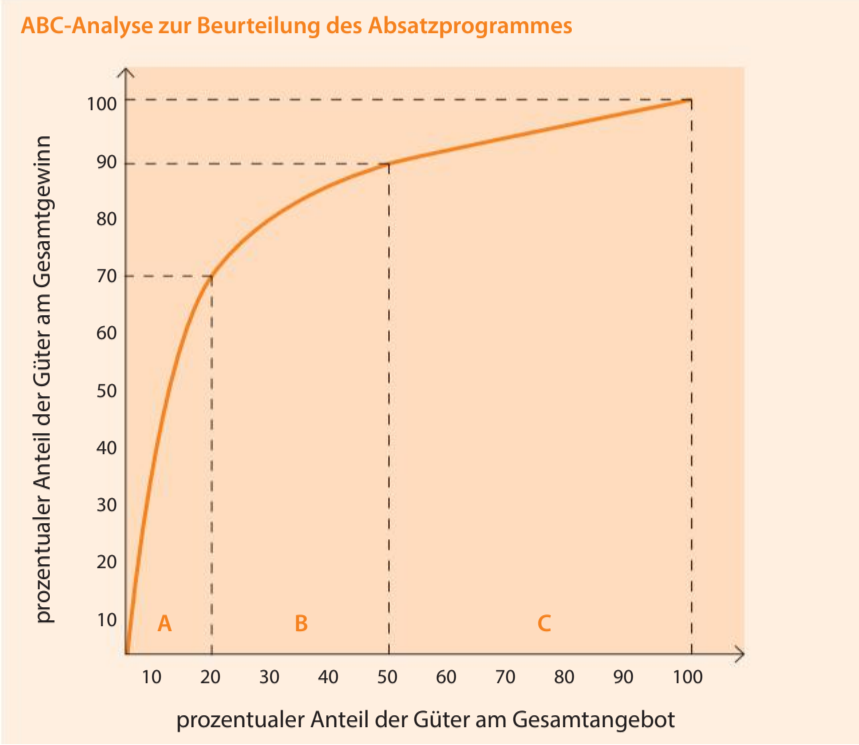
\includegraphics[scale=0.4]{ABC-Analyse.png}
    \end{center}
\end{figure}

\newpage
\subsection{Produktgestaltung}
\textbf{Produktgestaltung} umfasst alle Massnahmen, die zur Festlegung oder Veränderungen von Produkteigenschaften getroffen werden:
\begin{itemize}
    \item Produktinnovation
    \item Produktvariation
    \item Produktrelaunch
    \item Produktelimination
\end{itemize}
Die Gestaltung eines Produkts umfasst 3 Dimensionen:
\begin{figure}[h]
    \begin{center}
        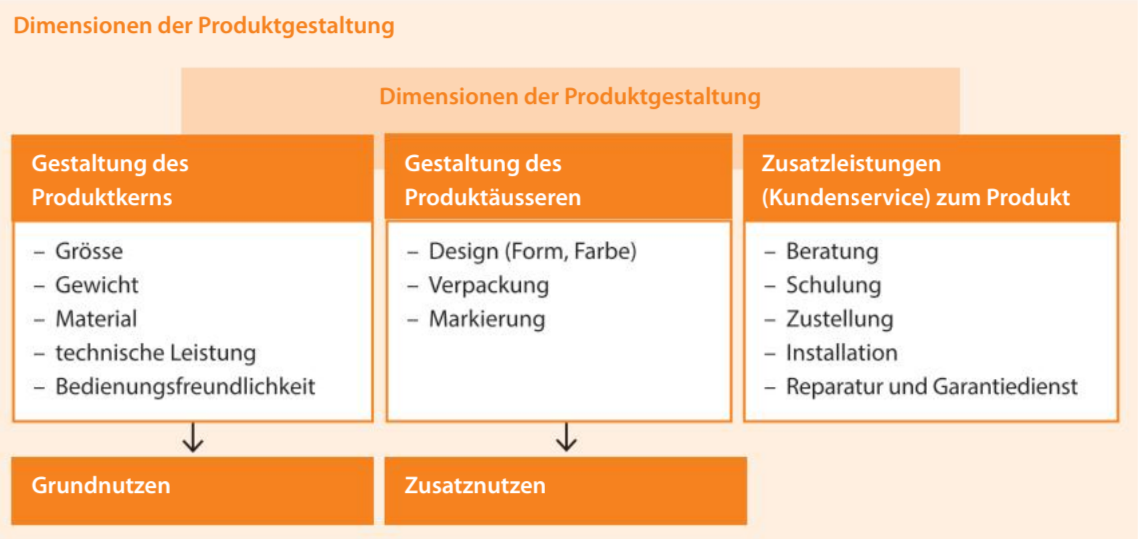
\includegraphics[scale=0.4]{Dimensionen der Produktgestaltung.png}
    \end{center}
\end{figure}

\section{Capaul: D9 Preispolitik}
\subsection{Aufgaben der Preispolitik}
\begin{Definitionsbox}
    Die \textbf{Preispolitik} umfasst alle Überlegungen und Entscheidungen, die den Preis eines Produkts betreffen. Sie beschäftigt sich mit der Preistbestimmung und -differenzierung.
\end{Definitionsbox}
Ziel ist die maximierung des Gewinns. Daraus lassen sich Unterziele ableiten:
\begin{itemize}
    \item Erhöhung des Umsatzes
    \item Erhöhung des Marktanteils
    \item Aufbau oder Stärkung eines bestimmten Images
    \item Kundengewinnung und Kundenbindung
\end{itemize}

\subsection{Preisbestimmung}
Orientierungspunkte bei der Preisbestimmung sind:
\begin{itemize}
    \item Zahlungsbereitschaft
    \item Kosten 
    \item Wettbewerb
\end{itemize}

\subsubsection{Preiselastizität}
\begin{Definitionsbox}
    Die \textbf{Preiselastizität der Nachfrage} $\varepsilon_p$ gibt an, wie die Nachfragemenge nach einem Gut auf Preisänderung reagiert.
\end{Definitionsbox}
\begin{equation}
    \varepsilon_p = \frac{\frac{M_2-M_1}{M_1}}{\frac{P_2-P_1}{P_1}} = \frac{\text{rel. Mengenänderung}}{\text{rel. Preisänderung}}
\end{equation}
$M$: Menge\\
$P$: Preis
\\[10pt]
Bei einer \textbf{preiselastischen Nachfrage}
\begin{equation*}
    \varepsilon_p < -1
\end{equation*}
wird die Nachfrage als elastisch bezeichnet. Die Konsumenten reagieren relativ empfindlich auf Preisänderungen.

Von \textbf{preisunelastischer Nachfrage} ist die Rede, wenn
\begin{equation*}
    0 < \varepsilon_p > -1
\end{equation*}
ist. Konsumenten reagieren in diesem Fall unempfindlich auf Preisänderungen.

\newpage
\textbf{Vollkommen preisunelastische Nachfrage} ist, wenn
\begin{equation*}
    \varepsilon_p = 0
\end{equation*}
gilt.

Von \textbf{inversen Preiselastizität der nachfrage (Snob-Effekt)} spricht man bei
\begin{equation*}
    \varepsilon_p > 0
\end{equation*}
. Dieser Verlauf der Nachfragekurve ist abnormal und spielt bei Gütern eine Rolle, die ienen hohe Prestigewert besitzen.

\subsubsection{Ankerpreis}
\begin{Definitionsbox}
    Ein \textbf{Ankerpreis} ist ein Referenzwert, den Kunden als Vergleichsmaßstab nutzen, um zu beurteilen, ob ein Preis hoch oder niedrig ist, unabhängig davon, ob dieser Anker rational ist oder nicht.
\end{Definitionsbox}

\subsubsection{Deckungsbeitragsanalyse}
Ein Unternehmen ist in der Preisgestaltung gegen unten nicht frei. Die Deckungsbeitragsanalyse signalisiert einem Unternehmen, welchen Preis es für ein Produkt mindestens erhalten muss.

Der \textbf{Deckungsbeitrag pro Stück} $db$ ergibt sich aus der Differenz zwischen dem Preis $p$ und den variablen Kosten $k_V$:
\begin{equation}
    db = p - k_v
\end{equation}
Der Deckungsbeitrag $db$ steht dem Unternehmen zur Deckung der fixen Kosten $k_F$ zur Verfügung. Werden diese gedeckt, dann trägt der Deckungsbetrag zum Gewinn bei.

\subsubsection{Break-even-Analyse}
Mithilfe der \textbf{Break-even-Analyse} wird der kritische Stückpreis $x$ ermittelt, durch den die Durchschnittskosten gerade gedeckt sind.
\begin{equation}
    x = \frac{K_f}{p - k_v}
\end{equation}
Die Auflösung nach dem Preis $p$ führt zu einer allgemeinen Formel für den Break-even-Preis $P$.
\begin{equation}
    P = \frac{K_f}{x} + k_v
\end{equation}

\subsubsection{Zuschlagverfahren}
Beim \textbf{Zuschlagverfahren} wird zu den Kosten eines Produkts (Break-even-Preis) ein bestimmter Gewinnzuschlag addiert.
\begin{equation}
    \text{Verkaufspreis} = \text{Stückkosten in CHF} + \text{Gewinnzuschlag}
\end{equation}

\subsubsection{Leitpreisverfahren}
Alternativ zum Zuschlagverfahren bietet sich der Leitpreis für die Preisbildung an. Bei dieser Preisbestimmung richtet sich ein Unternehmen nach den Preisen der Konkurrenz.
\begin{equation}
    \text{Leitpreis (Verkaufspreis)} - k_v = db
\end{equation}

\subsection{Preispolitische Strategien}
\begin{Definitionsbox}
    Bei der \textbf{Preisdifferenzierung} bietet ein Unternehmen das gleiche produkt oder die gleiche Dienstleistung verschiedenen Nachfragern zu unterschiedlichen Preisen am Markt an.
\end{Definitionsbox}

\subsection{Konditionenpolitik}



\end{document}